\section{Beugung}

\subsubsection{Terminologie}

Die \textbf{Richtungsänderungen} der Wellenausbreitung in einem homogenen Medium durch \textbf{Hindernisse} wird als \textbf{Beugung (Diffraction)} bezeichnet.

\smallskip

\begin{itemize}
	\item Das Hindernis kann eine Kante, ein Spalt oder ein kleines Objekt sein 
	\item Beugung tritt auf, wenn das \textbf{Hindernis} von \textbf{ähnlicher Grösse} ist, wie die \textbf{Wellenlänge} 
\end{itemize}

\smallskip

\textrightarrow\ \textbf{Beugung tritt auf, wenn eine Welle limitiert wird!}

\medskip

Dies gilt insbesondere für: 
Spalt, Kante, Loch (Pinhole), Objektiv-Öffnung


\subsection{Beugung -- Spalt}

\subsubsection{Beschreibung Setup}\label{Beschreibung Setup}

\begin{center}
    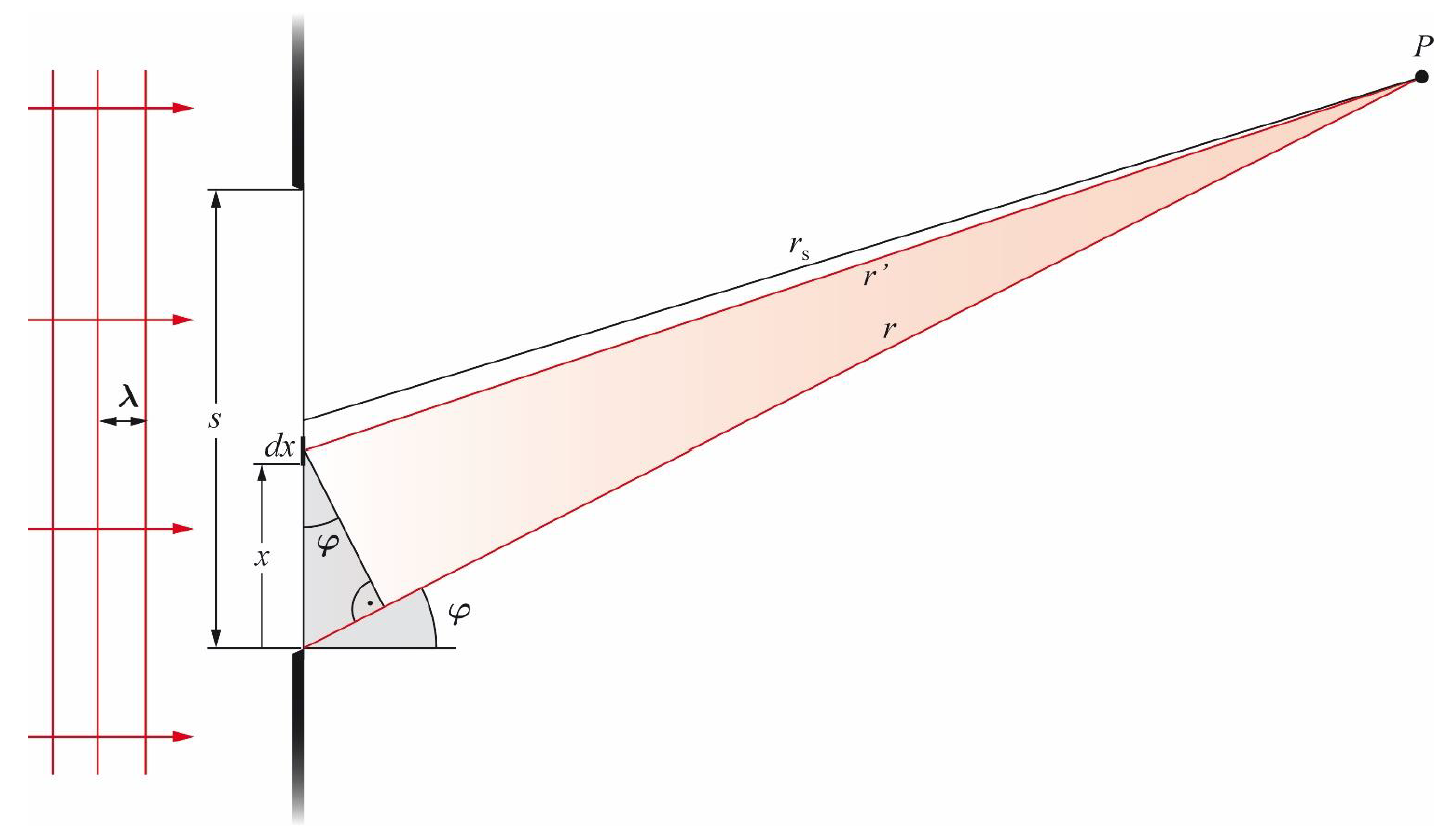
\includegraphics[width=0.7\columnwidth]{images/beugung_spalt.png}
\end{center}


\subsubsection{Intensität nach dem Spalt}

\begin{minipage}[t]{0.58\columnwidth}
    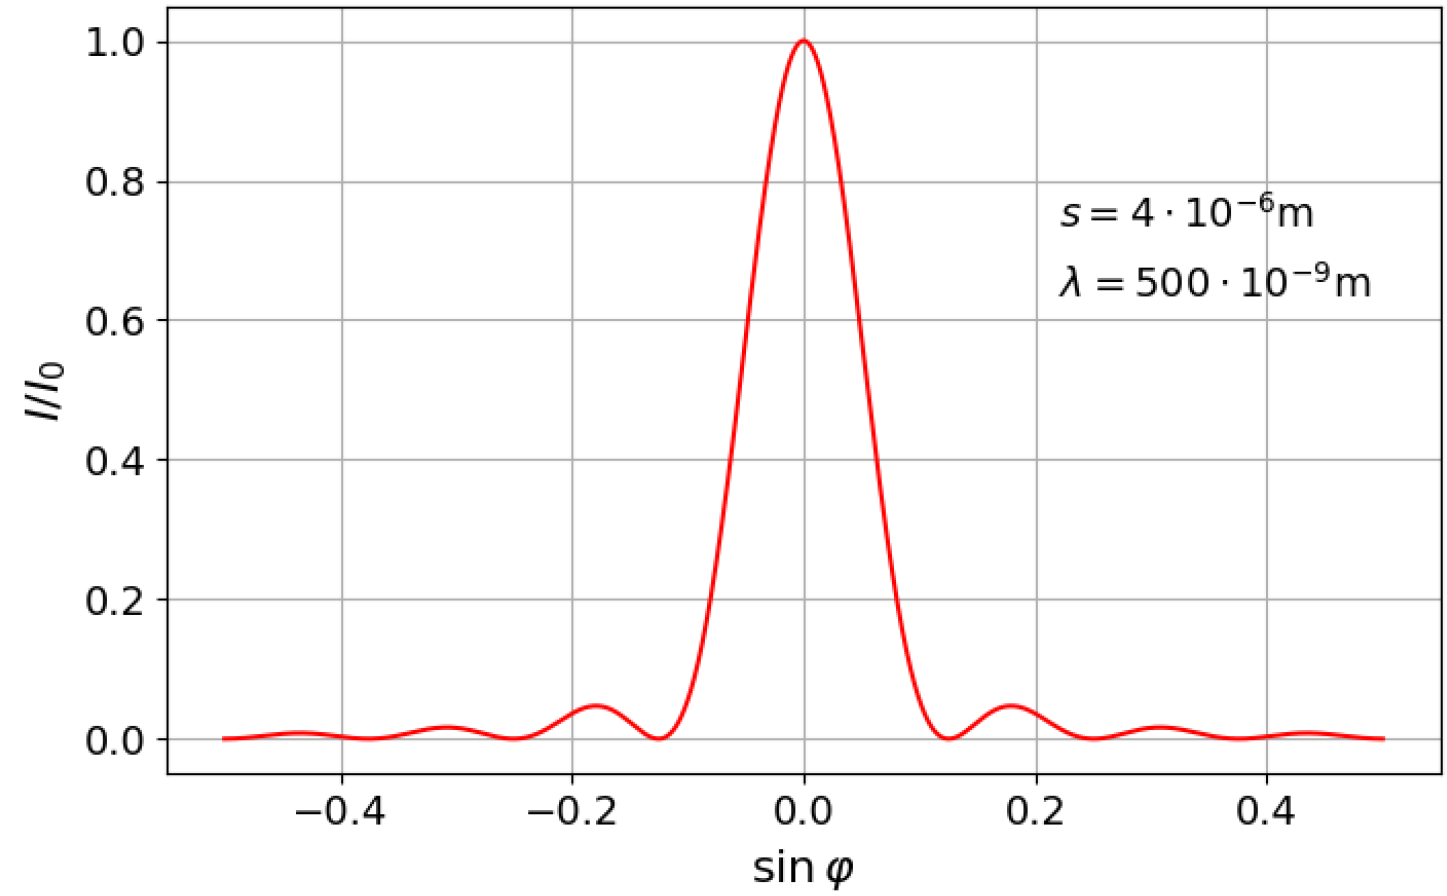
\includegraphics[width=\columnwidth, align=t]{images/beugung_spalt_intensitaet.png}
\end{minipage}
\hfill
\begin{minipage}[t]{0.4\columnwidth}
    $$ \boxed{ I_s \varpropto \frac{A^2}{r^2} \frac{\sin^2\left( \frac{k \cdot s \cdot \sin(\varphi)}{2} \right) }{\left( \frac{k \cdot s \cdot \sin(\varphi)}{2} \right) } } $$

    \smallskip

    \paragraph{Minima der Intensität} 
    $$ \boxed{ \sin(\varphi) = n \, \frac{\lambda}{s}} $$
\end{minipage}

\renewcommand{\arraystretch}{1.2}
\begin{ctabular}{clc}
    $I_s$       & Intensität                                                            & $[I_s] = \frac{W}{\meter\squared}$    \\
    $s$         & Länge des Spalts                                                      & $[s] = \meter$                        \\
    $\lambda$   & Wellenlänge                                                           & $[\lambda]= \meter$                   \\
    $n$         & Ordnung (typ. 1)                                                      & $[n] = 1$                             \\
    $A$         & Amplitude                                                             & $[A]$                                 \\
    $r$         & siehe Bild Abschnitt \ref{Beschreibung Setup}                         & $[r] = \meter$                        \\
    $\varphi$   & Einfallswinkel der Welle zum Spalt                                    & $[\varphi] =$°                        \\
                & \cbl{Hinweis: Oft muss gegebenes $\varphi$ durch 2 geteilt werden!}   &                                       \\
    % & \cbl{geteilt werden!}
\end{ctabular}
\renewcommand{\arraystretch}{1}


\subsection{Beugung -- Runde Öffnung (2D)}

\begin{minipage}[t]{0.48\columnwidth}
    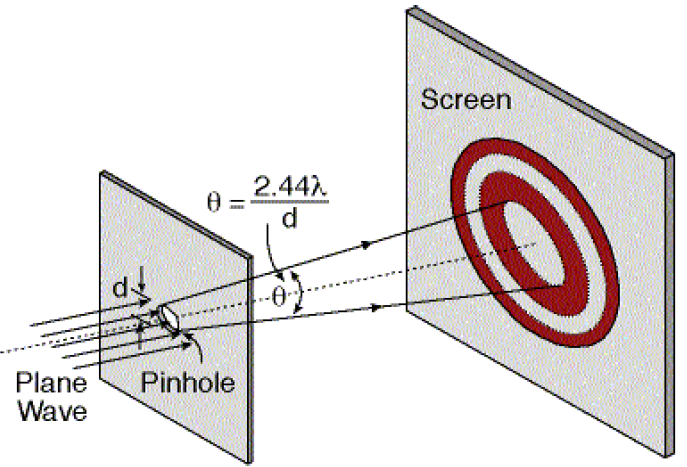
\includegraphics[width=\columnwidth, align=t]{images/beugung_loch.png}
\end{minipage}
\hfill
\begin{minipage}[t]{0.48\columnwidth}
    \paragraph{Nullstelle erster Ordnung} 
    $$ \boxed{ \sin(\varphi) = 1.22 \frac{\lambda}{D} } $$ 

    \renewcommand{\arraystretch}{1.2}
    \begin{ctabular}{clc}
        $\lambda$   & Wellenlänge       & $[\lambda]= \meter$ \\
        $D$         & Loch-Durchmesser  & $[D] = \meter$
    \end{ctabular}
    \renewcommand{\arraystretch}{1}
\end{minipage}


\subsection{Beugung -- Gitter}

\subsubsection{Beschreibung Setup}

\begin{center}
    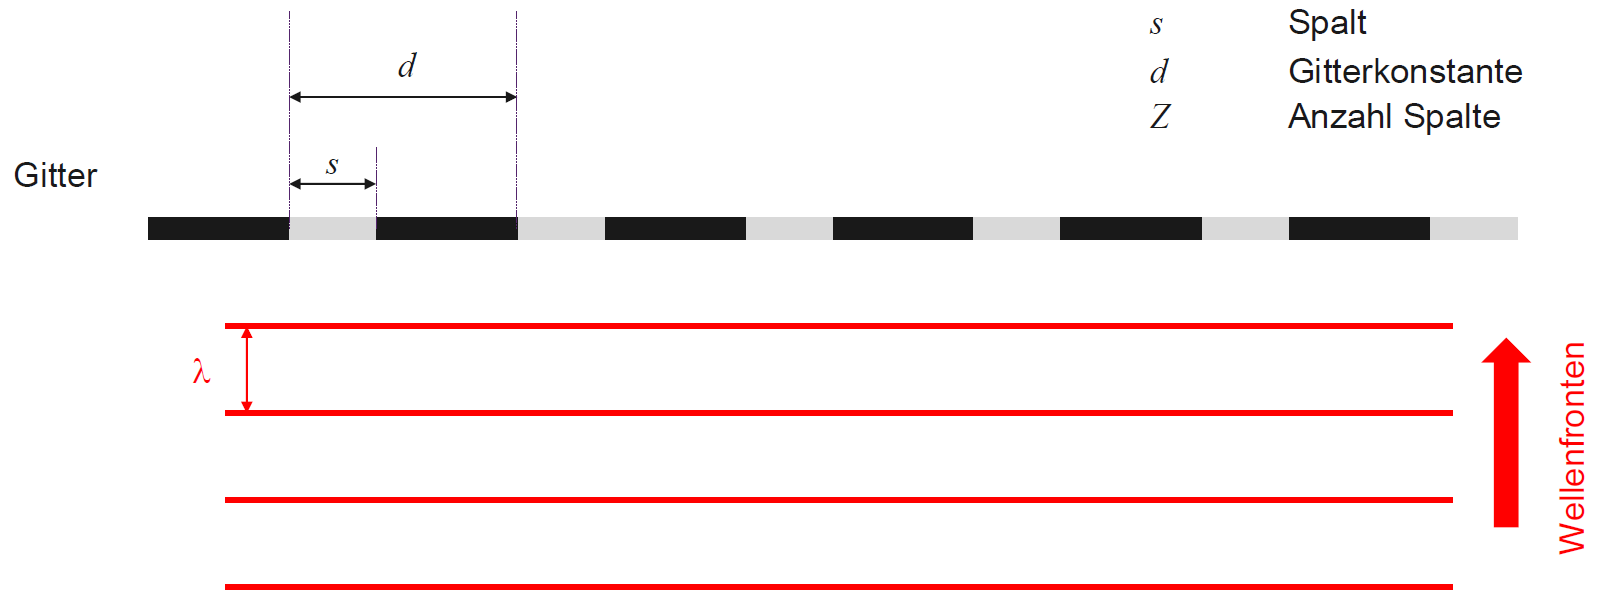
\includegraphics[width=0.85\columnwidth]{images/beugung_gitter.png}
\end{center}


\subsubsection{Intensität nach dem Gitter}

$$ \boxed{ I_G = \frac{A^2}{r^2} \textcolor{red}{A_s^2} \, \textcolor{green}{B^2} } $$

\begin{center}
    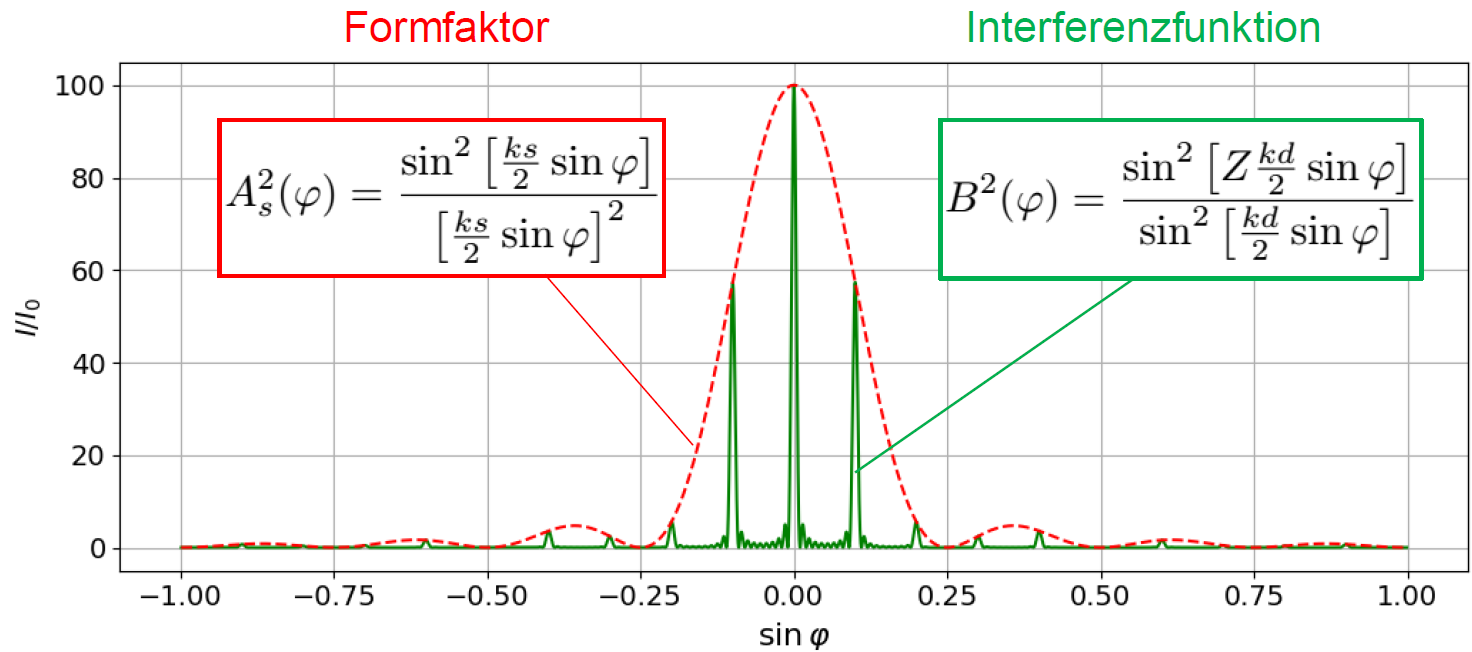
\includegraphics[width=0.9\columnwidth]{images/beugung_gitter_intensitaet.png}
\end{center}


\resizebox{\columnwidth}{!}{
    \renewcommand{\arraystretch}{1.3}
    \begin{tabular}{@{}ll@{}}
        $A_s^2(\varphi)$    & hat Nullstellen bei $n \, \frac{\lambda}{s}$ (hängt von $s$ ab) \\
        $B^2(\varphi)$      & hat Hauptmaxima bei $n \, \frac{\lambda}{d}$ und $Z - 2$ Nebenmaxima dazwischen (hängt von $Z$ und $d$ ab)
    \end{tabular}
    \renewcommand{\arraystretch}{1}
}

\renewcommand{\arraystretch}{1.3}
\begin{ctabular}{clc}
    $I_G$   & Intensität nach Gitter    & $[I_G] = \frac{W}{\meter\squared}$    \\
    $k$     & Wellenzahl                & $[k] = \frac{1}{\meter}$              \\
    $s$     & Spalt                     & $[s] = \meter$                        \\
    $d$     & Gitterkonstante           & $[d] = \meter$                        \\
    $Z$     & Anzahl Spalte             & $[Z] = 1$
\end{ctabular}
\renewcommand{\arraystretch}{1}


\subsubsection{Auflösungsvermögen}

Verschiedene Wellenlängen können getrennt (aufgelöst) werden

\begin{center}
    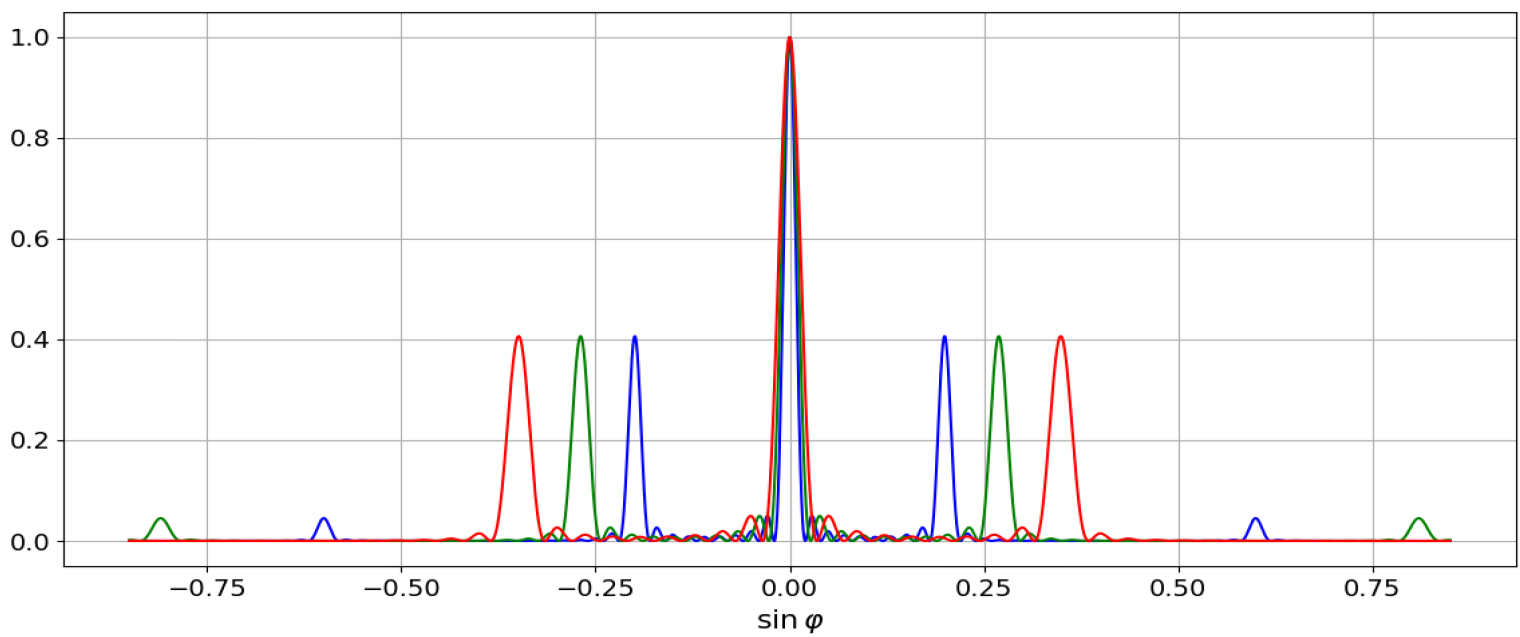
\includegraphics[width=0.9\columnwidth]{images/aufloesungsvermoegen.png}
\end{center}


\paragraph{Kriterium}


Zwei Wellenlängen werden gerade noch aufgelöst, wenn das Hauptmaximum von $\lambda_2$ mit dem Minimum von $\lambda_1$ zusammenfällt

$$ \boxed{ \frac{\lambda}{\Delta \lambda} = n \, Z } $$

\renewcommand{\arraystretch}{1.3}
\begin{ctabular}{clc}
    $\lambda$           & Wellenlänge                   & $[\lambda] = \meter$          \\
    $\Delta \lambda$    & Unterschied der Wellenlängen  & $[ \Delta \lambda] = \meter$  \\
    $n$                 & Ordnung der Beugung (typ. 1)  & $[n] = 1$                     \\
    $Z$                 & Anzahl der Spalten            & $[Z] = 1$ 
\end{ctabular}
\renewcommand{\arraystretch}{1}


\subsection{Babinet-Prinzip}

\begin{minipage}[t]{0.48\columnwidth}
    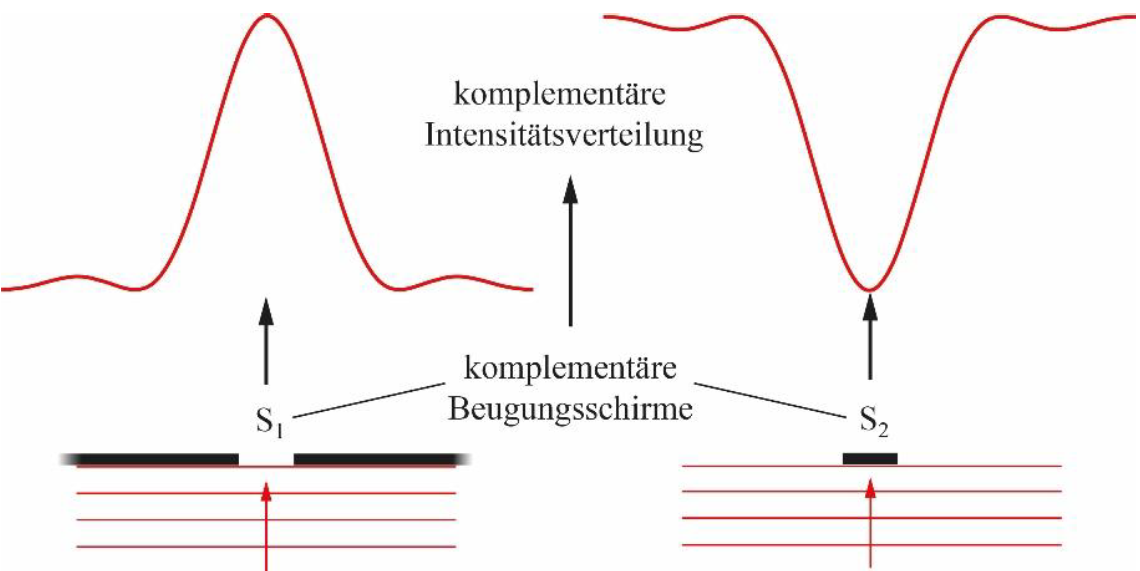
\includegraphics[width=\columnwidth, align=t]{images/babinet_prinzip.png}
\end{minipage}
\hfill
\begin{minipage}[t]{0.48\columnwidth}
    \raggedright%
    Ausserhalb des Bereichs geometrisch-optischer Abbildung produzieren komplementäre Beugungsschirme gleiche Beugungsbilder
\end{minipage}

